
%(BEGIN_QUESTION)
% Copyright 2012, Tony R. Kuphaldt, released under the Creative Commons Attribution License (v 1.0)
% This means you may do almost anything with this work of mine, so long as you give me proper credit

Et {\it burner management system} (BMS) overvåker flammetilstanden ved bunnen av denne forbrenningsenheten, for å sikre at brenngass ikke fortsetter inn i forbrenningskammeret uten etablert flamme:

$$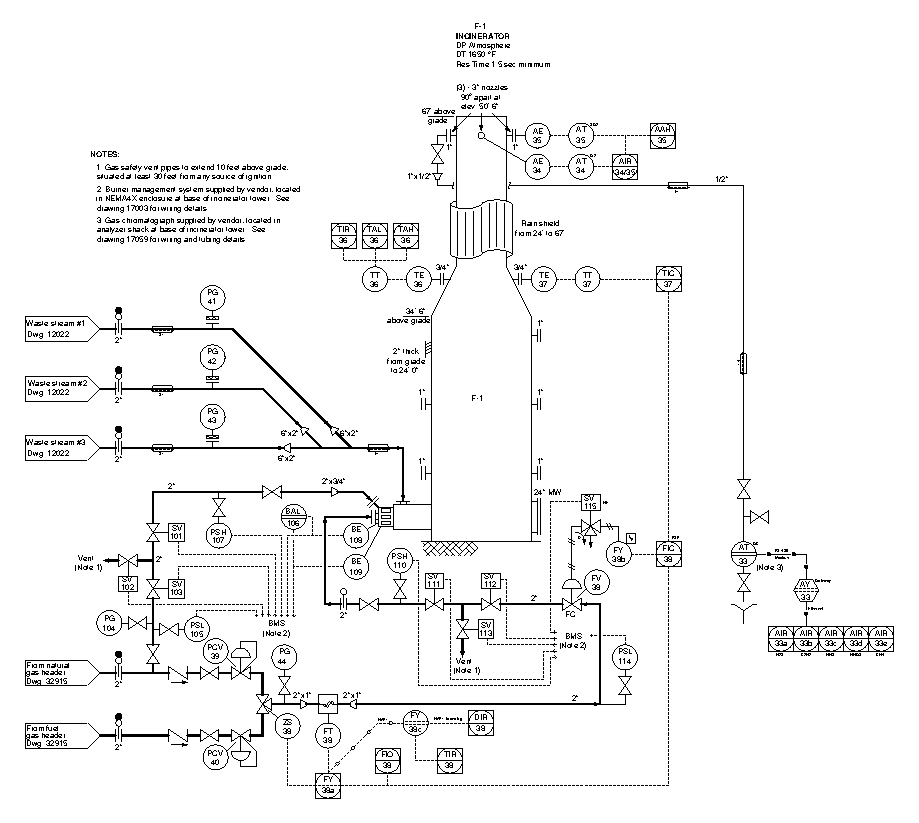
\includegraphics[width=15.5cm]{i0004rx01.eps}$$

Forklar funksjonen til magnetventil SV-115, og oppgi om den er normalt energisert (NE) eller normalt av-energistert (NDE).

\vskip 20pt \vbox{\hrule \hbox{\strut \vrule{} {\bf Forslag til sokratisk diskusjon} \vrule} \hrule}

\begin{itemize}
\item{} Er det mulig å fastslå ``normal'' energiseringsstatus for magnetventilene SV-111, SV-112 og/eller SV-113 ut fra diagrammet? Forklar hvorfor eller hvorfor ikke.
\item{} Forklar hva som kan skje i systemet hvis magnetventil SV-111 feiler.
\item{} Forklar hva som kan skje i systemet hvis magnetventil SV-103 feiler.
\item{} Forklar hva som kan skje i systemet hvis magnetventil SV-113 feiler.
\item{} Forklar hva som kan skje i systemet hvis magnetventil SV-102 feiler.
\end{itemize}

\underbar{file i00866}
%(END_QUESTION)





%(BEGIN_ANSWER)


%(END_ANSWER)





%(BEGIN_NOTES)

SV-115 er normalt energisert, og tvinger FV-38 til sin feilsikre (stengte) posisjon dersom BMS detekterer flammeutfall.

\vskip 10pt

Vi kan ikke bestemme energiseringstilstandene til SV-111, SV-112 eller SV-113 fra dette diagrammet alene, fordi vi ikke ser hvilken ventiltilstand som faktisk er gjennomslipp versus blokkering.









\vskip 20pt \vbox{\hrule \hbox{\strut \vrule{} {\bf Virtual feilsøking} \vrule} \hrule}

Denne oppgaven egner seg godt som en ``Virtual Troubleshooting''-øvelse. Når diagrammet vises for studentene, kan du først tenke ut en bestemt feil i systemet. Deretter presenterer du ett eller flere symptomer på feilen (noe en operatør eller annen bruker kan observere). Studentene foreslår så diagnostiske tester for å identifisere feilens art og plassering, som om de faktisk feilsøkte anlegget. Din oppgave er å oppgi hvilke resultater testene ville gitt, og dokumentere dem synlig for alle.

Under og etter øvelsen er det nyttig å stille oppfølgingsspørsmål som:

\begin{itemize}
\item{} Hva forteller resultatet av siste diagnostiske test om feilen?
\item{} Hvis resultatet av siste diagnostiske test hadde vært annerledes, hva ville det fortalt om feilen da?
\item{} Er siste diagnostiske test den beste testen vi kunne gjort?
\item{} Hva ville vært ideell testrekkefølge for å diagnostisere problemet med færrest mulige trinn?
\end{itemize}


%INDEX% Final Control Elements, valve: fail-safe solenoids
%INDEX% Process: incinerator (realistic P\&ID shown)

%(END_NOTES)
